In this section we present the algorithm \AlgJakub\ that yields a discrepancy of roughly $\ln(4) \approx 1.39$ for large $k$. Compared to the algorithm \AlgKarl\ from the last section, \AlgJakub\ has a considerably better discrepancy at the price of a more involved analysis, and it only works for $k$ being a power of two. 

\begin{theorem} \label{thm:algjacub}
  For $k\ge 8$ being any power of 2, the algorithm \AlgJakub\ has discrepancy
\LV{\[    
  \Perf(\AlgJakub) \le \ln(4) + \frac{0.05}{\lg(k/4)} + O\Big(\frac1{k}\Big).
  \]
}\SV{\[
  \Perf(\AlgJakub) \le \ln(4) + 0.05/\lg(k/4) + O\left(k^{-1}\right)
\]}
\end{theorem}
Here and in the remainder of this paper, let `$\lg$' denote the binary and `$\ln$' the natural logarithm. Note that the term $O(1/k)$ quickly tends to 0, whereas the $\Theta(1/\lg(k/4))$ term is small due to the constant $0.05$. Hence, this discrepancy is close to $\ln(4)$ already for moderate $k$. Also note that $\ln(4)$ is by less than $0.1$ larger than our lower bound from Sect.~\ref{sec:lower_bound}, leaving room for less than a $6\%$ improvement over\LV{ the upper bound for} algorithm \AlgJakub\ for large $k$. 
\LV{We verified experimentally that algorithm \AlgJakub\ yields very good bounds already for relatively small $k$. The results are summarized in Fig.~\ref{fig:jakubs_algorithm_performance}.}

\subsection{The Algorithm \AlgJakub} 

The initial checkpoints $t_1,\ldots,t_k$ satisfy the equation
\begin{equation} \label{eq:tialpha}
  t_i = \alpha t_{i/2} 
\end{equation}
for each even $1 \le i \le k$ and some $\alpha = \alpha(k) \ge 2$. Precisely, we set
\[
  \alpha := 2^{1 + \frac{\lg(\sqrt{2}/\ln 4)}{\lg(k/4)} } \approx 2^{1+ \frac{0.029}{\lg(k/4)}}.
\]
However, the usefulness of this expression becomes clear only in the analysis\LV{ of the algorithm}.

During one period we delete all odd checkpoints $t_1,t_3,\ldots,t_{k-1}$ and insert\LV{ the new checkpoints}
\begin{equation} \label{eq:newti}
  t_{k+i} := \alpha t_{k/2+i},
\end{equation}
for $1 \le i \le k/2$. Then after one period we end up with the checkpoints
\[
\begin{array}{l*{5}{l@{,\,}}@{\quad}*{3}{l@{,\ }}ll}
  &(t_2 & t_4 & \ldots\, & t_{k-2} & t_k & t_{k+1} & t_{k+2} &\ldots\, & t_{k+k/2})&  \\
  = \alpha \cdot&(t_1 & t_2 & \ldots\, & t_{k/2-1} &t_{k/2} & t_{k/2+1} & t_{k/2+2} & \ldots\, &t_{k/2+k/2})& = \alpha (t_1,t_2,\ldots,t_k),
\end{array}
\]
which proves cyclicity. Note that~\eqref{eq:tialpha} and~\eqref{eq:newti} allow us to compute all $t_i$ from the values $t_{k/2+1},\ldots,t_k$, however, we still have some freedom to choose the latter values. Without loss of generality we can set $t_k := 1$, then $t_{k/2} = \alpha^{-1}$. In between these two values, we interpolate $\lg t_i$ linearly, i.e., we set for $i \in (k/2,k]$
\begin{equation} \label{eq:tiinterpol}
  t_i := \alpha^{2i/k - 2},
\end{equation}
completing the definition of the $t_i$. Note that\LV{ this equation}\SV{\eqref{eq:tiinterpol}} also works for $i=k$ and $i=k/2$.

\LV{There is one more freedom we have with this algorithm, namely in which order we delete all odd checkpoints during one period, i.e., we need to fix the pattern of removals.}
In iteration $1 \le i \le k/2$ we insert the checkpoint $t_{k+i}$ and remove the checkpoint $t_{d(i+k)}$, defined as follows. For $m \in \N = \N_{\ge 1}$ let $2^{e(m)}$ be the largest power of 2 that divides $m$. We define $S \colon \N \to \N, S(m) := m / 2^{e(m)}$. Note that $S(m)$ is an odd integer. Using this definition, we set
\LV{\begin{equation} \label{eq:defd}
  d(k+i) := S\Big(i+ \frac k2 \Big),
\end{equation}}
\SV{\begin{equation}\label{eq:defd}
  d(k+i) := S(i+k/2)
\end{equation}}
finishing the definition of the algorithm \AlgJakub. If we write this down as a pattern, then we have $p_i = 1 + k/(2^{1+e(i)})$ for $1 \le i < k/2$ and $p_{k/2} = 1$.
For intuition as to the behavior of this pattern, see the example in Fig.~\ref{fig:jakubs_algorithm_movement}.
\LV{
The following lemma implies that the deletion behavior of \AlgJakub\ is indeed well-defined, meaning that during one period we delete all odd checkpoints $t_1,t_3,\ldots,t_{k-1}$ (and no point is deleted twice).
\begin{lemma}
  The function $S$ induces a bijection between $\{k/2 < i \le k\}$ and $\{1 \le i \le k \mid i \text{ is odd} \}$.
\end{lemma}
\begin{proof}
  Let $A := \{k/2 < i \le k\}$ and $B := \{1 \le i \le k \mid i \text{ is odd} \}$.
  Since $S(m) \le m$ and $S(m)$ is odd for all $m \in \N$, we have $S(A) \subseteq B$. Moreover, $A$ and $B$ are of the same size. We present an inverse function to finish the proof. Let $x \in B$. Note that there is a unique number $y \in \N$ such that $x 2^y \in A$, since $A$ is a range between two consecutive powers of 2 and $x \le k$. Setting $S^{-1}(x) = x 2^y$ we have found the inverse. ~
\end{proof}
}\SV{It is not hard to see that with $d$ as defined above, we indeed delete all odd checkpoints $t_1,t_3,\ldots,t_{k-1}$ during one period,
in the full version of this paper we include a formal proof of this.}
\begin{figure}
  \centering
  \definecolor{gray}{RGB}{178,178,178}
    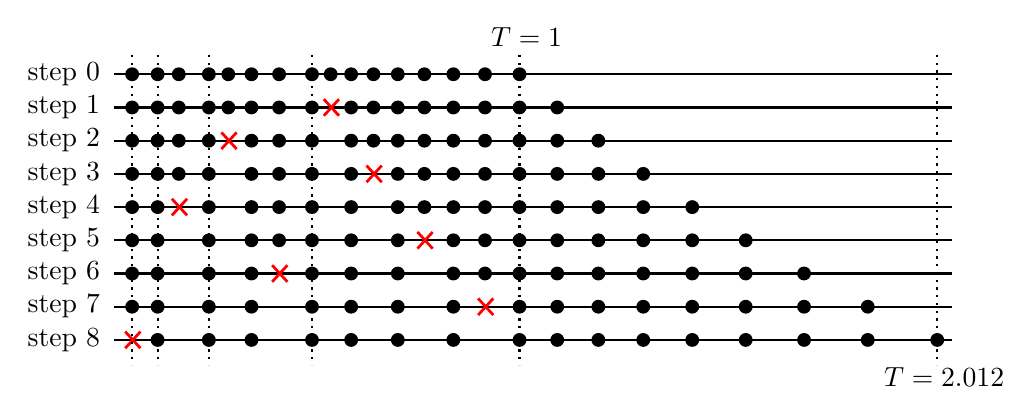
\begin{tikzpicture}[y=1pt, x=1pt,yscale=-1, inner sep=0pt, outer sep=0pt]
    \def\linespread{\baselineskip}
    \foreach \i in {0,1,2,...,8} {
      \path[shift={(0,0)}, draw=black, line join=miter, line cap=butt, line width=0.8pt]
        (0,\i * \linespread) node[left=5] {step \i} -- (303, \i * \linespread) ;
    }
    \foreach \x in {9.086718622889968, 18.28737691914821, 25.94320242291756, 36.80406189100548, 43.83609267359075, 52.211710397032434, 62.18762978904628, 74.06961521412411, 80.83661709068994, 88.22185242594281, 96.28180304394778, 105.07811094961241, 114.67804976293608, 125.155039223504, 136.58920670012435, 149.068} {
      \path[fill=black]
              (\x,0)arc(0.000:180.000:2.500)arc(-180.000:0.000:2.500) -- cycle;
    }
    \draw (149.068,0) node [above=10] {$T=1$};

    \foreach \x in {9.086718622889968, 18.28737691914821, 25.94320242291756, 36.80406189100548, 43.83609267359075, 52.211710397032434, 62.18762978904628, 74.06961521412411, 88.22185242594281, 96.28180304394778, 105.07811094961241, 114.67804976293608, 125.155039223504, 136.58920670012435, 149.068, 162.6868561641611} {
      \path[fill=black]
              (\x,\linespread )arc(0.000:180.000:2.500)arc(-180.000:0.000:2.500) -- cycle;
    }
    \foreach \x in {9.086718622889968, 18.28737691914821, 25.94320242291756, 36.80406189100548, 52.211710397032434, 62.18762978904628, 74.06961521412411, 88.22185242594281, 96.28180304394778, 105.07811094961241, 114.67804976293608, 125.155039223504, 136.58920670012435, 149.068, 162.6868561641611, 177.549931364065} {
      \path[fill=black]
              (\x,2*\linespread)arc(0.000:180.000:2.500)arc(-180.000:0.000:2.500) -- cycle;
    }
    \foreach \x in {9.086718622889968, 18.28737691914821, 25.94320242291756, 36.80406189100548, 52.211710397032434, 62.18762978904628, 74.06961521412411, 88.22185242594281, 105.07811094961241, 114.67804976293608, 125.155039223504, 136.58920670012435, 149.068, 162.6868561641611, 177.549931364065, 193.7708974815676} {
      \path[fill=black]
              (\x,3*\linespread)arc(0.000:180.000:2.500)arc(-180.000:0.000:2.500) -- cycle;
    }
    \foreach \x in {9.086718622889968, 18.28737691914821, 36.80406189100548, 52.211710397032434, 62.18762978904628, 74.06961521412411, 88.22185242594281, 105.07811094961241, 114.67804976293608, 125.155039223504, 136.58920670012435, 149.068, 162.6868561641611, 177.549931364065, 193.7708974815676, 211.47381146446045} {
      \path[fill=black]
              (\x,4*\linespread)arc(0.000:180.000:2.500)arc(-180.000:0.000:2.500) -- cycle;
    }
    \foreach \x in {9.086718622889968, 18.28737691914821, 36.80406189100548, 52.211710397032434, 62.18762978904628, 74.06961521412411, 88.22185242594281, 105.07811094961241, 125.155039223504, 136.58920670012435, 149.068, 162.6868561641611, 177.549931364065, 193.7708974815676, 211.47381146446045, 230.79406410635147} {
      \path[fill=black]
              (\x,5*\linespread)arc(0.000:180.000:2.500)arc(-180.000:0.000:2.500) -- cycle;
    }
    \foreach \x in {9.086718622889968, 18.28737691914821, 36.80406189100548, 52.211710397032434, 74.06961521412411, 88.22185242594281, 105.07811094961241, 125.155039223504, 136.58920670012435, 149.068, 162.6868561641611, 177.549931364065, 193.7708974815676, 211.47381146446045, 230.79406410635147, 251.87941550709863} {
      \path[fill=black]
              (\x,6*\linespread)arc(0.000:180.000:2.500)arc(-180.000:0.000:2.500) -- cycle;
    }
    \foreach \x in {9.086718622889968, 18.28737691914821, 36.80406189100548, 52.211710397032434, 74.06961521412411, 88.22185242594281, 105.07811094961241, 125.155039223504, 149.068, 162.6868561641611, 177.549931364065, 193.7708974815676, 211.47381146446045, 230.79406410635147, 251.87941550709863, 274.8911251329348} {
      \path[fill=black]
              (\x,7*\linespread)arc(0.000:180.000:2.500)arc(-180.000:0.000:2.500) -- cycle;
    }
    \foreach \x in {18.28737691914821, 36.80406189100548, 52.211710397032434, 74.06961521412411, 88.22185242594281, 105.07811094961241, 125.155039223504, 149.068, 162.6868561641611, 177.549931364065, 193.7708974815676, 211.47381146446045, 230.79406410635147, 251.87941550709863, 274.8911251329348, 300.0051851189134} {
      \path[fill=black]
              (\x,8*\linespread)arc(0.000:180.000:2.500)arc(-180.000:0.000:2.500) -- cycle;
    }

    \draw (300.00518511, 8*\linespread) node [below=10pt] {$T=2.012$};

    \foreach \i/\x in {1/80.8366170907, 2/43.8360926736, 3/96.2818030439, 4/25.9432024229, 5/114.678049763, 6/62.187629789, 7/136.5892067, 8/9.08671862289} {
      \path[draw=red, line width = 1pt] 
        (\x - 5, \i * \linespread - 3) -- (\x + 0.5 , \i  * \linespread + 3);
      \path[draw=red, line width = 1pt]
        (\x - 5, \i * \linespread + 3) -- (\x + 0.5, \i  * \linespread - 3);
    }
    \foreach \x in {9.086718622889968, 18.28737691914821, 36.80406189100548, 74.06961521412411, 149.068, 300.0051851189134} {
      \path[draw=black, dotted, line width = 0.8pt]
        (\x -2.5, -7) -- (\x -2.5, 8*\linespread + 9);
    }
\end{tikzpicture}
\caption{One period of the algorithm \AlgJakub\ for $k=16$. Note that, recursively, checkpoints are removed twice as often from the right half of the initial setting \LV{(at steps $i$ where $i \mod 2=1$) }as from the second quarter. }
\label{fig:jakubs_algorithm_movement}
\end{figure}

\subsection{Discrepancy Analysis} 
We now bound the largest discrepancy encountered during one period, i.e.,
\[
  \Perf(\AlgJakub) = \max_{1 \le i \le k/2} q(\AlgJakub,t_{i+k}) = (k+1) \max_{1 \le i \le k/2} \overline{\ell}_{t_{i+k}} / t_{i+k}.
\]
\SV{

  By Lemma~\ref{lem:only_new_intervals}, we only have to consider intervals newly created by insertion and deletion at any step. We do this exemplarily for the intervals from insertion.
}\LV{

  We first compute the maximum and later multiply with the factor $k+1$.
  By Lemma~\ref{lem:only_new_intervals}, we only have to consider intervals newly created by insertion and deletion at any step.

}
\paragraph{Intervals from Insertion:}
We \LV{first }compute the discrepancy of the interval newly added at time $t_{i+k}$, $1 \le i \le k/2$. Its length is $t_{i+k} - t_{i+k-1}$, so its discrepancy \LV{(without the factor $k+1$) }is
  \begin{align*}
    \SV{(k+1)} \frac{t_{i+k} - t_{i+k-1}}{t_{i+k}}
    &= \SV{(k+1) \left(} 1 - \frac{t_{i+k-1}}{t_{i+k}} \SV{\right)}  \\
    &= \SV{(k+1) \left(} 1 - \frac{ t_{i+k/2-1} }{ t_{i+k/2} } \SV{\right)} \LV{\\}
    \LV{&}\stackrel{\eqref{eq:tiinterpol}}{=} \SV{(k+1) \left(} 1 - \alpha^{-2/k} \SV{\right)},
  \end{align*}
  where the second equality holds because of \eqref{eq:newti} if $i>1$ or \eqref{eq:tialpha} if $i=1$.

  Using $e^x \ge 1+x$ for $x \in \mathbb{R}$ yields a bound on the discrepancy of 
  \[
    \SV{(k+1) }\frac{t_{i+k} - t_{i+k-1}}{t_{i+k}} \le \SV{(k+1)} \ln(\alpha) \frac{2}{k} = \ln(\alpha^2)\SV{ + O(k^{-1})}.
  \]
 \SV{ Since we choose $\alpha \approx 2$, we obtain a discrepancy of roughly $\ln(4)$, and the error term can easily be seen to be bounded by $0.05/\ln(k/4) + O(k^{-1})$. }

\LV{

\paragraph{Deleting $t_1$:} 
We show similar bounds for the intervals we get from deleting an old checkpoint. We first analyze the deletion of $t_1$---this case is different from the general one, since $t_1$ has no predecessor. Note that $t_1$ is deleted at time $t_{3k/2}$. The deletion of $t_1$ creates the interval $[0,t_2]$. This interval has discrepancy
\begin{align*}
  \frac{t_2}{t_{3k/2}} 
  \stackrel{\eqref{eq:newti},\eqref{eq:tialpha}}{=} \frac{\alpha t_1}{\alpha t_k}
  \stackrel{\eqref{eq:tialpha}}{=} \alpha^{-\lg k} \le 1/k,
\end{align*}
since we choose $\alpha \ge 2$. Hence, this discrepancy is dominated by the one we get from newly inserted intervals.


\paragraph{Other Intervals from Deletion:} 
It remains to analyze the discrepancy of the intervals we get from deletion in the general case, i.e., at some time $t_{i+k}$, $1 \le i < k/2$. At this time we delete checkpoint $d(i+k)$, so we create the interval $[t_{d(i+k)-1},t_{d(i+k)+1}]$ of discrepancy
\[
  q_i := \frac{ t_{d(i+k)+1} - t_{d(i+k)-1} }{ t_{i+k} }
  \stackrel{\eqref{eq:newti},\eqref{eq:defd}}{=} \frac{ t_{S(i+k/2)+1} - t_{S(i+k/2)-1} }{ \alpha t_{i+k/2} }.
\]
Let $h := e(i+k/2)$, so that $2^h$ is the largest power of 2 dividing $i+k/2$, and $2^h \,S(i+k/2) = i+k/2$. Then $t_{S(i+k/2)+1} = \alpha^{-h} t_{i+k/2+2^h}$ by \eqref{eq:tialpha}, and a similar statement holds for $t_{S(i+k/2)-1}$, yielding
\[
  q_i = \alpha^{-1-h} \frac{ t_{i+k/2+2^h} - t_{i+k/2-2^h} }{ t_{i+k/2} }.
\]
Using \eqref{eq:tiinterpol} we get $t_{i+k/2} = \alpha^{2i/k - 1}$. Comparing this with the respective terms for $t_{i+k/2+2^h}$ and $t_{i+k/2-2^h}$ yields
\begin{align*}
  q_i &= \alpha^{-1-h} \left(\alpha^{2^{h+1}/k} - \alpha^{-2^{h+1}/k}\right) \\
  &= \alpha^{-1-h} \cdot 2 \sinh \left( \ln \left(\alpha^2\right) 2^h / k \right).
\end{align*}
By elementary means one can show that the function $f(x) = x^{-A} \sinh(B x)$, $A \ge 1, B > 0$, is convex on $\mathbb{R}_{\ge 0}$. Since convex functions have their maxima at the boundaries of their domain, and since by above equation $q_i$ can be expressed using $f(2^h)$ (for $A = \lg \alpha$ and $B = \ln(\alpha^2)/k$), we see that $q_i$ is maximal at (one of) the boundaries of $h$. Recall that we treated $i=k/2$ separately, and observe that the largest power of 2 dividing $i+k/2$, $1 \le i < k/2$ is at most $k/4$. Hence, we have $0 \le 2^h \le k/4$ and 
\[
  q_i \le \max\left\{ 2 \alpha^{-1} \sinh(\ln(\alpha^2)/k), 2 \alpha^{-1} (k/4)^{-\lg \alpha} \sinh( \ln(\alpha)/2) \right\}.
\]
We simplify using $\alpha \ge 2$ and $\sinh(x) = x + O(x^2)$ to get
\begin{equation} \label{eq:jakubsqi}
  q_i \le \max\left\{ \ln(\alpha^2)/k + O(1/k^2), (k/4)^{-\lg \alpha} \sinh( \ln(\alpha)/2) \right\}.
\end{equation}
The first term is already of the desired form. For the second one, note that setting $\alpha = 2$ we would get a discrepancy of $4 \sinh(\ln(2)/2) / k = \sqrt{2}/k$. We get a better bound by choosing
\[
  \alpha := 2^{1 + \frac{c}{\lg(k/4)} },
\]
with $c := \lg( \sqrt{2} / \ln(4)) \approx 0.029$.
Then the second bound on $q_i$ from above becomes
\[
  (k/4)^{-\lg \alpha} \sinh( \ln(\alpha)/2) = \frac 4k 2^{-c} \sinh\left( \frac{\ln(2)}{2} \Big(1+\frac{c}{\lg(k/4)}\Big)\right).
\]
The particular choice of $c$ allows to bound the derivative of $\sinh((1+x) \ln(2)/2)$ for $x \in [0,c]$ from above by 
\[
  \frac{\ln(2)}{2} \cosh((1+c) \ln(2)/2) < 0.39.
\]
Hence, we can upper bound 
\[
  \sinh\left( \frac{\ln(2)}{2} \Big(1+\frac{c}{\lg(k/4)}\Big)\right) \le \sinh(\ln(2)/2) + \frac{0.39 c}{\lg(k/4)}.
\]
Thus, in total the second bound on $q_i$ from inequality~(\ref{eq:jakubsqi}) becomes 
\[
  (k/4)^{-\lg \alpha} \sinh( \ln(\alpha)/2) 
  \le  \frac 4k 2^{-c} \sinh(\ln(2)/2) + \frac{4 \cdot 2^{-c} \cdot 0.39 c}{k \lg(k/4)}.
\]
Since $c = \lg( \sqrt{2} / \ln(4)) = \lg( 4 \sinh(\ln(2)/2) / \ln(4) )$, this becomes 
\[
  \le \ln(4)/k + 0.044 / (k \lg(k/4)).
\]

\paragraph{Overall discrepancy:} 
In total, we can bound the discrepancy $q := \Perf(\AlgJakub)$ of our algorithm (now including the factor of $k+1$) by
\[
  q \le (k+1) \max\left\{ \ln(\alpha^2)/k + O(1/k^2), \ln(4)/k + 0.044/(k \lg(k/4)) \right\}.
\]
Using $(k+1)/k = 1 + O(1/k)$ and 
\[
  \ln(\alpha^2) = \ln(4) \left( 1 + \frac{c}{\lg(k/4)} \right) \le \ln(4) + \frac{0.040}{\lg(k/4)},
\]
this bound can be simplified to
\[
  q \le \max\{ \ln(4) + 0.040/\lg(k/4) + O(1/k), \ln(4) + 0.044/\lg(k/4) + O(1/k) \},
\]
which proves Theorem~\ref{thm:algjacub}.
}
